\documentclass{beamer}
\usepackage{tikz}
\usepackage{xcolor}

\definecolor{darkgreen}{rgb}{0.0, 0.7, 0.13}
\setbeamertemplate{navigation symbols}{}%remove navigation symbols

\begin{document}

\begin{frame}
%\frametitle{Genetic distance = rate $\times$ time}
%\framesubtitle{Relaxed molecular clock}

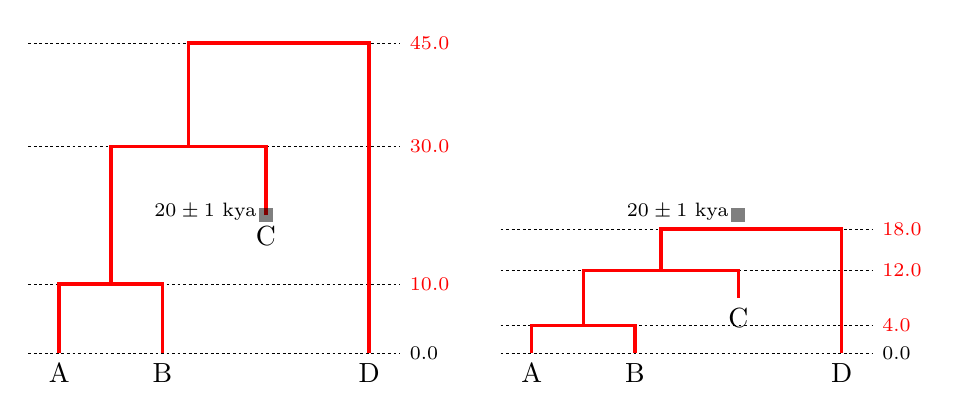
\begin{tikzpicture}[yscale=-0.8,xscale=0.8]
  
  \draw[dash pattern=on 1.0 off 1.0 ] (-14pt, 140pt) -- (154pt, 140pt);
  \node[anchor=west, dash pattern=on 1.0 off 1.0 ] at (154pt, 140pt) {\scriptsize{0.0}};
  \draw[dash pattern=on 1.0 off 1.0 ] (-14pt, 108.88889pt) -- (154pt, 108.88889pt);
  \node[red,anchor=west, dash pattern=on 1.0 off 1.0 ] at (154pt, 108.88889pt) {\scriptsize{10.0}};
  \draw[dash pattern=on 1.0 off 1.0 ] (-14pt, 46.66667pt) -- (154pt, 46.66667pt);
  \node[red,anchor=west, dash pattern=on 1.0 off 1.0 ] at (154pt, 46.66667pt) {\scriptsize{30.0}};
  \draw[dash pattern=on 1.0 off 1.0 ] (-14pt, 0pt) -- (154pt, 0pt);
  \node[red,anchor=west, dash pattern=on 1.0 off 1.0 ] at (154pt, 0pt) {\scriptsize{45.0}};
  \node[anchor=north, line width=1.25pt] at (0pt, 140pt) {A};
  \node[anchor=north, line width=1.25pt] at (46.66667pt, 140pt) {B};
  \draw[line width=1.25pt,red] (0pt, 140pt) -- (0pt, 108.88889pt) -- (23.33333pt, 108.88889pt);
  \draw[line width=1.25pt,red] (46.66667pt, 140pt) -- (46.66667pt, 108.88889pt) -- (23.33333pt, 108.88889pt);
  \node[anchor=north, line width=1.25pt] at (93.33334pt, 77.77778pt) {C};
  \draw[line width=1.25pt,red] (23.33333pt, 108.88889pt) -- (23.33333pt, 46.66667pt) -- (58.33333pt, 46.66667pt);
  \draw[line width=1.25pt,red] (93.33333pt, 77.77778pt) -- (93.33333pt, 46.66667pt) -- (58.33333pt, 46.66667pt);
  \node[anchor=north, line width=1.25pt] at (140pt, 140pt) {D};
  \draw[line width=1.25pt,red] (58.33333pt, 46.66667pt) -- (58.33333pt, 0pt) -- (99.16667pt, 0pt);
  \draw[line width=1.25pt,red] (140pt, 140pt) -- (140pt, 0pt) -- (99.16667pt, 0pt);
  
  \draw[line width=5, black,opacity=0.5] (93.33334pt,74.666666pt) -- (93.33334pt,80.888888pt);
  
  %\draw[black,dash pattern=on 1.0 off 1.0 ] (-14pt,31.111111pt) -- (58.33333pt,31.111111pt); 
  %\draw[black,dash pattern=on 1.0 off 1.0 ] (-14pt,62.22222pt) -- (58.33333pt,62.22222pt); 
  \node[anchor=east] at (93.33334pt, 76pt) {\scriptsize{$20 \pm 1$ kya}};

  \begin{scope}[xshift=7.5cm,yshift=84pt,yscale=0.4]
  \draw[dash pattern=on 1.0 off 1.0 ] (-14pt, 140pt) -- (154pt, 140pt);
  \node[anchor=west, dash pattern=on 1.0 off 1.0 ] at (154pt, 140pt) {\scriptsize{0.0}};
  \draw[dash pattern=on 1.0 off 1.0 ] (-14pt, 108.88889pt) -- (154pt, 108.88889pt);
  \node[red,anchor=west, dash pattern=on 1.0 off 1.0 ] at (154pt, 108.88889pt) {\scriptsize{4.0}};
  \draw[dash pattern=on 1.0 off 1.0 ] (-14pt, 46.66667pt) -- (154pt, 46.66667pt);
  \node[red,anchor=west, dash pattern=on 1.0 off 1.0 ] at (154pt, 46.66667pt) {\scriptsize{12.0}};
  \draw[dash pattern=on 1.0 off 1.0 ] (-14pt, 0pt) -- (154pt, 0pt);
  \node[red,anchor=west, dash pattern=on 1.0 off 1.0 ] at (154pt, 0pt) {\scriptsize{18.0}};
  \node[anchor=north, line width=1.25pt] at (0pt, 140pt) {A};
  \node[anchor=north, line width=1.25pt] at (46.66667pt, 140pt) {B};
  \draw[line width=1.25pt,red] (0pt, 140pt) -- (0pt, 108.88889pt) -- (23.33333pt, 108.88889pt);
  \draw[line width=1.25pt,red] (46.66667pt, 140pt) -- (46.66667pt, 108.88889pt) -- (23.33333pt, 108.88889pt);
  \node[anchor=north, line width=1.25pt] at (93.33334pt, 77.77778pt) {C};
  \draw[line width=1.25pt,red] (23.33333pt, 108.88889pt) -- (23.33333pt, 46.66667pt) -- (58.33333pt, 46.66667pt);
  \draw[line width=1.25pt,red] (93.33333pt, 77.77778pt) -- (93.33333pt, 46.66667pt) -- (58.33333pt, 46.66667pt);
  \node[anchor=north, line width=1.25pt] at (140pt, 140pt) {D};
  \draw[line width=1.25pt,red] (58.33333pt, 46.66667pt) -- (58.33333pt, 0pt) -- (99.16667pt, 0pt);
  \draw[line width=1.25pt,red] (140pt, 140pt) -- (140pt, 0pt) -- (99.16667pt, 0pt);

  \end{scope}
  
    \begin{scope}[xshift=7.5cm]
  \draw[line width=5, black,opacity=0.5] (93.33334pt,74.666666pt) -- (93.33334pt,80.888888pt);
  \node[anchor=east] at (93.33334pt, 76pt) {\scriptsize{$20 \pm 1$ kya}};
 \end{scope}

\end{tikzpicture}
\end{frame}
\end{document}